\documentclass{beamer}
\usepackage{etex}
\usetheme{Antibes}
\usepackage{amssymb,amsmath,amsthm}
\usepackage{graphicx}
\usepackage{caption}
\usepackage{subfig}
\newcommand{\bn}{\begin{enumerate}[i)]}
\newcommand{\en}{\end{enumerate}}
\newcommand{\im}{\item}
\newcommand{\CPT}[1]{\large{\textbf{CHAPTER #1}}}
\newcommand{\ir}[1]{\textbf{Remark #1}}
\newcommand{\ith}[1]{\textbf{Theorem #1}}
\newcommand{\idf}[1]{\textbf{Definition #1}}
\newcommand{\iex}[1]{\textbf{Example #1}}

%\definecolor{cardinal}{rgb}{0.77, 0.12, 0.23}
%\usecolortheme[named=cardinal]{structure}
%\setbeamercolor{block title}{bg=cardinal,fg=black}
 \usepackage{tikz}
 \usetikzlibrary{patterns,snakes,plotmarks}
 \usepackage{multirow}
% \usetikzlibrary{shadows}
\usepackage{epstopdf}
\usepackage{nicefrac}
\usepackage{lmodern}
\usepackage{pgfplots}
\usepackage{qtree}
\newcommand*{\Scale}[2][4]{\scalebox{#1}{\ensuremath{#2}}}%
\DeclareCaptionLabelSeparator{horse}{:\,\,} % change according to your needs
\captionsetup{
  labelsep = horse,
  figureposition = bottom % used to get the correct vertical space between the figure and the caption
}
\setbeamertemplate{caption}[numbered]
\setbeamertemplate{items}[circle]
\setbeamertemplate{enumerate items}[square]
\theoremstyle{definition}
\newtheorem*{exs}{Examples}
\newtheorem{ex}{Example}
\newtheorem*{exc}{Exercise}
%\usepackage{booktabs}
\setlength{\parindent}{0pt}
%\setbeameroption{show notes}
 \setbeamerfont{note page}{size=\tiny}
%\setbeamertemplate{note page}[plain]
%\setbeameroption{show only notes}
\title{Math 629 - Survival Analysis \\ Chapter 5: The Stratified Cox Procedure}
\author{Drew Lazar}
\institute{Ball State University}
\date{\today}

\begin{document}
\begin{frame}
    \titlepage
\end{frame}



\section{Chapter 5}
\begin{frame}
\frametitle{The Stratified Cox Procedue}
\begin{block}{Overview}
\begin{enumerate}
\item We can deal with variables that don't satifisy the PH assumption by stratification.
\item We will see stratification by a single covariate and more than one covariate.
\item We will consider a stratified Cox PH model without and with interaction.
\end{enumerate}
\end{block}
\end{frame}

\begin{frame}
\frametitle{Stratification by covariate without interaction}
\begin{block}{Example 5.1: Remission data - stratification by Sex}
\begin{itemize}
\item We saw in chapter 4 that in the Remission data set: TR and LogWBC statisfy the PH assumption but Sex does not.
\item We can stratify on Sex (Male and Female) and create Cox PH models using TR and LogWBC in each strata. Without interaction we have:
\[
h_g(t,X) = h_{0,g}(t)\exp(\beta_1 TR + \beta_2 logWBC) \text{ for } g=1,2.
\]
\item $g$ denotes the stratum with $g=1$ for Females and $g=2$ for Males.
\item With no interaction, for both stratum the effect of a unit increase of a covariate on the hazard (HR) is the same.
\end{itemize}
\end{block}
\end{frame}

\begin{frame}
\frametitle{Stratification by covariate without interaction (cont'd)}
\begin{block}{Problem 5.1: Remission data - stratification by Sex}
\begin{enumerate}
\item In R, fit a stratified Cox PH model to the Remission Data. Use TR and LogWBC as covariates and stratify on Sex.
\item Use a Wald test to test for the significance of TR and LogWBC.
\item Use a Likelihood ratio test to 1) test for the significance of TR and logWBC and 2) test for the significance of TR with LogWBC in the model.
\item Interpret the coefficients of TR and LogWBC in the stratified Cox PH model.
\item Plot adjusted survival curves for TR from your Stratified Cox PH model. Set logWBC=mean(logWBC).
\end{enumerate}
\end{block}
\end{frame}

\begin{frame}
\frametitle{Stratification by covariate without interaction (cont'd)}
\begin{block}{The General Statified Cox (SC) Model}
\begin{enumerate}
\item We describe the general form of the SC model that allows for stratification of several predictors.
\item We have $k$ variables not satisfying the PH assumption and $p$ variables satisfying the PH assumption.
\item $Z_1, Z_2,. . ., Z_k$ do not satisfy PH. $X_1, X_2,. . ., X_p$ satisfy PH.
\item We proceed as follows:
\begin{enumerate}
\item Categorize each $Z_i$.
\item Form $k^*$ combinations of categories.
\item The strata are the categories of $Z^*$.
\end{enumerate}
\end{enumerate}
\end{block}
\end{frame}

\begin{frame}
\frametitle{Stratification by covariate without interaction (cont'd)}
\begin{block}{The General Statified Cox (SC) Model (cont'd)}
Example with age and treatment. Age is interval variable so we stratify it.
   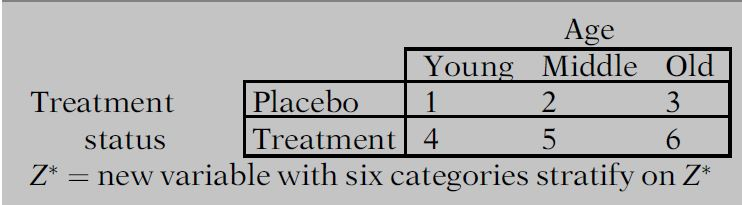
\includegraphics[width =\textwidth, height=4cm]{CH5_exampleSC}
\end{block}
\end{frame}

\begin{frame}
\frametitle{Stratification by covariate without interaction (cont'd)}
\begin{block}{The General Statified Cox (SC) Model (cont'd)}
\begin{enumerate}
\item The general SC model:
\begin{equation} \label{SCnoint}
h_g(t,X) = h_{0g}(t)exp(\beta_1 X_1 + \ldots + \beta_p X_p) \text{ for }  g=1,\ldots,k^*
\end{equation}
\item Different baseline hazard functions: $h_{0,g}(t), g=1,\ldots,k^*$ but same coefficients $\beta_1, \ldots, \beta_p$.
\item Without interaction, the effect of a unit increase of a covariate, $X_i$, on the hazard (i.e., the HR) is $\exp(\beta_i)$.
\end{enumerate}
\end{block}
\end{frame}

\begin{frame}
\frametitle{Stratification by covariate without interaction (cont'd)}
\begin{block}{The General Statified Cox (SC) Model (cont'd): Maximum Likelihood Estimation}
\begin{itemize}
\item We obtain estimates for $\beta_1,\ldots,\beta_p$ by partial maximum likelihood estimation.
\item We maximize a partial likelihood function, $L$, that is obtained by multiplying together likelihood functions for each
stratum as shown below.
\vspace{10pt}
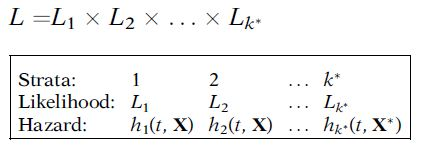
\includegraphics[width =\textwidth, height=3.2cm]{CH5_Partiallike}
\end{itemize}
\end{block}
\end{frame}


\begin{frame}
\frametitle{Stratification by covariate with interaction}
\begin{block}{Example 5.2: Remission data - stratification by Sex with interaction}
\begin{itemize}
\item Without interaction our SC model is
\[
h_g(t,X) = h_{0,g}(t)\exp(\beta_1 TR + \beta_2 logWBC) \text{ for } g=1,2.
\]
\item With interaction our SC model is
\begin{equation} \label{eq:Int1}
h_g(t,X) = h_{0,g}(t)\exp(\beta_{1g} TR + \beta_{2g} logWBC) \text{ for } g=1,2.
\end{equation}
\item With interaction the HR's depend on the strata. For example, with interaction the effect of a unit increase in TR on the hazard is
\[
\exp(\beta_{1g}) \text{ for } g=1,2.
\]
\end{itemize}
\end{block}
\end{frame}

\begin{frame}
\frametitle{Stratification by covariate with interaction (cont'd)}
\begin{block}{Example 5.2: Remission data - stratification by Sex with interaction (cont'd)}
\begin{itemize}
\item An alternative interaction model is a follows:
\begin{equation}\label{eq:Int2}
\begin{aligned}
h_g(t,X) & = h_{0,g}(t)\exp[\beta_1^* TR + \beta_2^* logWBC +  \\
& \beta_3^*(Sex*TR) + \beta_4^*(Sex*logWBC) ] \text{ for } g=1,2.
\end{aligned}
\end{equation}
\item Stratified interaction models \eqref{eq:Int1} and \eqref{eq:Int2} are, in fact, equivalent models.
\end{itemize}
\end{block}
\end{frame}

\begin{frame}
\frametitle{Stratification by covariate with interaction (cont'd)}
\begin{block}{Example 5.2: Remission data - stratification by Sex with interaction (cont'd)}
How are \eqref{eq:Int1} and \eqref{eq:Int2} equivalent?
\begin{itemize}
\item Using model \eqref{eq:Int1}, the natural log an effect of a unit increase in TR, i.e., ln[HR(TR)], is:
\[ \beta_{11} \text{ for } g=1 \text{ and }  \beta_{12} \text{ for } g=2.
\]
\item Using model \eqref{eq:Int2}, natural log the effect of a unit increase in TR, i.e., ln[HR(TR)], is:
\[
\beta_{1}^* + \beta_{3}^**\text{Sex}.
\]
\item Thus, $\beta_{11}=\beta_{1}^*$ and  $\beta_{12}=\beta_{1}^*+\beta_{3}^*$.
\item Similarily, we have $\beta_{21}=\beta_{2}^*$ and  $\beta_{22}=\beta_{2}^*+\beta_{4}^*$.
\end{itemize}
\end{block}
\end{frame}

\begin{frame}
\frametitle{Stratification by covariate with interaction (cont'd)}
\begin{block}{Problem 5.2: Remission data - stratification by Sex with interaction}
\begin{enumerate}
\item In R, fit a stratified Cox PH model to the Remission Data. Use TR and LogWBC as covariates and stratify on Sex. Assume interaction of the covariates with sex.
\item In R, test the interaction assumption using a likelihood ratio test at significance level $\alpha=0.05$.
\item Using the interaction model, find HR of TR for Sex=0 (female) and Sex=1 (male). Also find the $95\%$ CI's of these HR's.
\end{enumerate}
\end{block}
\end{frame}

\begin{frame}
\frametitle{Stratification by covariate with interaction (cont'd)}
\begin{block}{The General Stratified Cox (SC) Model with interaction}
\begin{enumerate}
\item $Z^*$ and $k^*$ as before.
\item The general SC model with interaction:
\begin{equation} \label{genSCint1}
h_g(t,X) = h_{0g}(t)exp(\beta_{1g} X_1 + \ldots + \beta_{pg} X_p) \text{ for }  g=1,\ldots,k^*
\end{equation}
\item Different baseline hazard functions: $h_{0,g}(t), g=1,\ldots,k^*$ and coefficients $\beta_{1g}, \ldots, \beta_{pg}$.
\item With interaction, the effect of a unit increase of a covariate, $X_i$, on the hazard (i.e., the HR) is $\exp(\beta_{ig})$ for $g=1,\ldots,k^*$ and depends on the strata $g$.
\end{enumerate}
\end{block}
\end{frame}

\begin{frame}
\frametitle{Stratification by covariate with interaction (cont'd)}
\begin{block}{The General Stratified Cox (SC) Model with interaction (cont'd)}
\begin{enumerate}
\item Let $Z^*$ and $k^*$ be as before and let $Z_1^*,\ldots,Z_{k*-1}$ be dummy variables representing the $k^*$ classes of $Z^*$.
\item Then the alternative General Stratified Cox (SC) Model with interaction is:
\begin{equation} \label{genSCint2}
\begin{aligned}
h_g&(t;X)= h_{0,g}\exp[\tilde{\beta}_1X_1 + \ldots + \tilde{\beta}_p X_p \\
&+\tilde{\beta}_{11}Z_1^*\times X_1 + \ldots + \tilde{\beta}_{p1}Z_1^*\times X_p \\
&+\tilde{\beta}_{12}Z_2^*\times X_1 + \ldots + \tilde{\beta}_{p2}Z_2^*\times X_p \\
&+\ldots \\
&+\tilde{\beta}_{1(k^*-1)}Z_{k^*-1}^*\times X_1 + \ldots + \tilde{\beta}_{p(k^*-1)}Z_{k^*-1}^*\times X_p]. \\
\end{aligned}
\end{equation}
\end{enumerate}
\end{block}
\end{frame}

\begin{frame}
\frametitle{Stratification by covariate with interaction (cont'd)}
\begin{block}{The General Stratified Cox (SC) Model with interaction (cont'd)}
\begin{itemize}
\item Model $\ref{genSCint1}$ and $\ref{genSCint2}$ are equivalent with
\[ \beta_{i1} = \tilde{\beta}_i \text{ and } \beta_{ig} = \tilde{\beta}_{i} + \tilde{\beta}_{i(g-1)} \text{ for } g=2,\ldots,k^*.
\]
\item For example 5.2 (Remission data) we have $g=2, k^*=2, X_1=\text{TR}, X_2=\text{logWBC}, Z_1^*=\text{Sex}$.
\begin{align*}
&h_g(t,X) = \beta_{1g} \exp( X_1 + \beta_{2g} X_2)  \text{ or } \\
&h_g(t,X) = h_{0,g}(t)\exp[\beta_1^*X_1  + \beta_2^*X_2 + \beta_3^*Z_1^*\times X_1 + \beta_4^*Z_1^*\times X_2 ]  \\
&\text{or } h_g(t,X) = h_{0,g}(t)\exp[\tilde{\beta}_1X_1  + \tilde{\beta}_2X_2 + \tilde{\beta}_{11}Z_1^*\times X_1 + \tilde{\beta}_{21}Z_1^*\times X_2 ]
\end{align*}
\end{itemize}
\end{block}
\end{frame}

\begin{frame}
\frametitle{Stratification by covariate with interaction (cont'd)}
\begin{block}{The General Stratified Cox (SC) Model with interaction (cont'd): likelihood ratio test for interaction}
\begin{itemize}
\item We can test for interaction of the covariates that satisfy the Cox PH model, $X_1,\ldots,X_p$ and $Z^*$.
\item $H_0: \tilde{\beta}_{ig} =0$ for $i=1,\ldots,p$ and $g=1,\ldots,k^*-1$.
\item We fit model \ref{SCnoint} as our reduced model and fit model \ref{genSCint2} as our full model.
\item Under $H_0$ our test statistic is approximately distributed as follows:
\[
CSStat= \-2(\ln(L_R) - \ln(L_F)) \sim \chi^2_{p(k^*-1)}.
\]
\item At significance level $\alpha$, we reject $H_0$  iff $CSStat>\chi^2_{\alpha,p(k^*-1)}$ or $p$-value$<\alpha$.
\end{itemize}
\end{block}
\end{frame}

\begin{frame}
\frametitle{Stratification by covariate with interaction}
\begin{block}{Example 5.3: Vets data set - stratification by cell type and performance status with interaction}
The dataset ``vets.dat'' considers survival times in days for 137 patients from the Veterans's Administration Lung Cancer Trial. The exposure variable of interest is treatment status.
The list of the variables is given as follows:
\begin{figure}
    \centering
    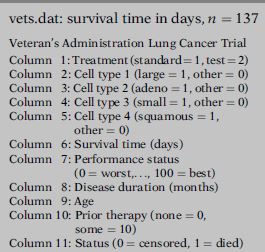
\includegraphics[height=3.5cm]{Ch5_vets.JPG}
  \end{figure}
\end{block}
\end{frame}

\begin{frame}
\frametitle{Stratification by covariate with interaction}
\begin{block}{Problem 5.3: Vets data set - stratification by cell type and performance status with interaction}
\begin{enumerate}
\item Use a GOF test with Schoenfeld residuals to determine which variables in the vets.dat data set satisfy the Cox PH model.
\item Fit a stratified Cox PH model stratifying on the variables that satisfy the PH assumption according to 1).
 \begin{enumerate}
 \item Fit a stratified model without interaction.
 \item Fit a stratified model with interaction.
\item Conduct a likelihood ratio test for interaction at significance level $\alpha=.05$.
\item Using the interaction model, determine the HR for Setting and the HR for Age when 1) the cell type is squamous and PSBin=0 and 2) the cell type is small and PSBin=1.
\end{enumerate}
\end{enumerate}
\end{block}
\end{frame}

\begin{frame}
\frametitle{Stratification by covariate with interaction}
\begin{block}{Problem 5.3: Vets data set - stratification by cell type and performance status with interaction (cont'd)}
\begin{columns}
    \begin{column}{0.48\textwidth}
        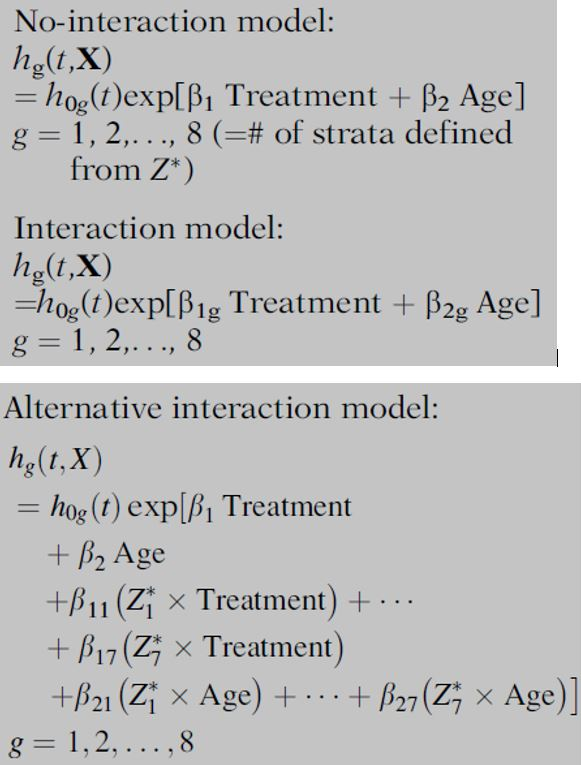
\includegraphics[width =\textwidth, height=6cm]{C5_models1.JPG}
    \end{column}
    \hspace{-10pt}
    \begin{column}{0.48\textwidth}
         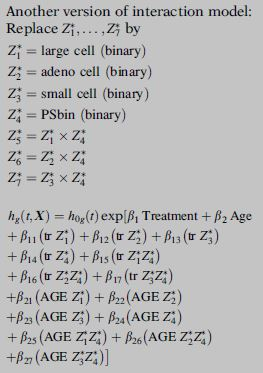
\includegraphics[width =\textwidth, height=6cm]{C5_models3.JPG}
    \end{column}
\end{columns}
\end{block}
\end{frame}

\begin{frame}
\frametitle{A Graphical View of the Stratified Cox Approach}
\begin{block}{Examples a. and b.}
\begin{columns}
    \begin{column}{0.48\textwidth}
        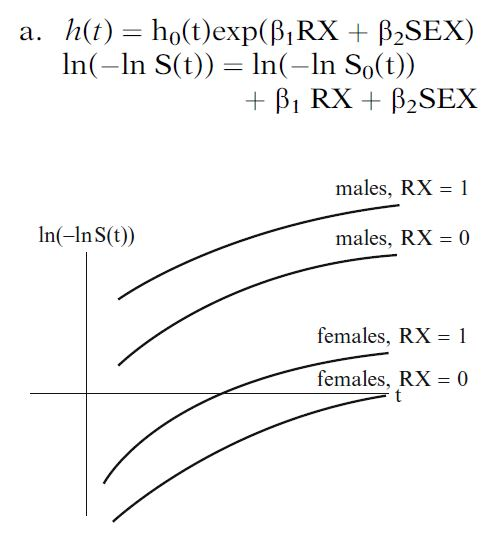
\includegraphics[width =\textwidth, height=5cm]{CH5_G1.JPG}
        a. No interaction and no stratification model.
    \end{column}
    \hspace{-10pt}
    \begin{column}{0.48\textwidth}
         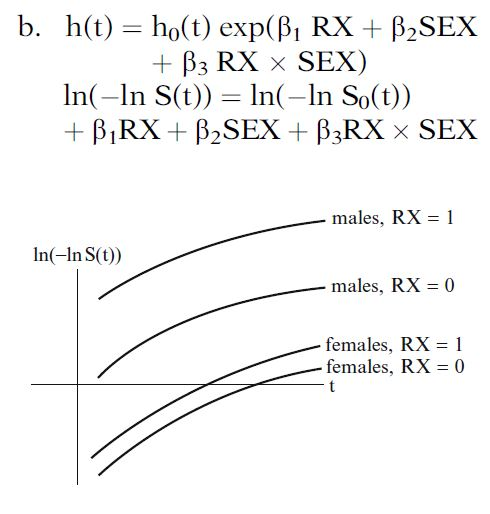
\includegraphics[width =\textwidth, height=5cm]{CH5_G2.JPG}
         a. Interaction and no stratification model.
    \end{column}
\end{columns}
\end{block}
\end{frame}

\begin{frame}
\frametitle{A Graphical View of the Stratified Cox Approach}
\begin{block}{Examples c. and d.}
\begin{columns}
    \begin{column}{0.48\textwidth}
        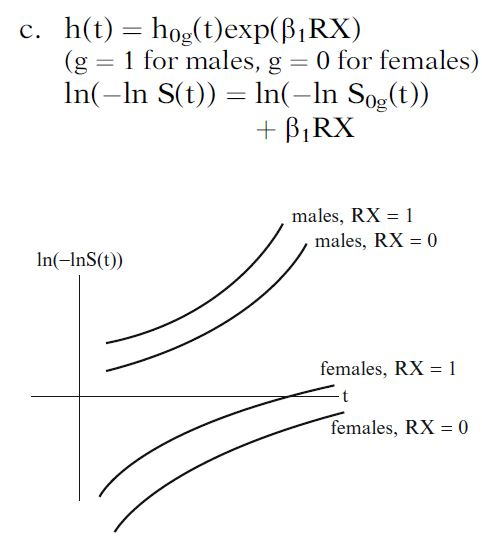
\includegraphics[width =\textwidth, height=5cm]{CH5_G3.JPG}
        c. No interaction and stratification model.
    \end{column}
    \hspace{-10pt}
    \begin{column}{0.48\textwidth}
         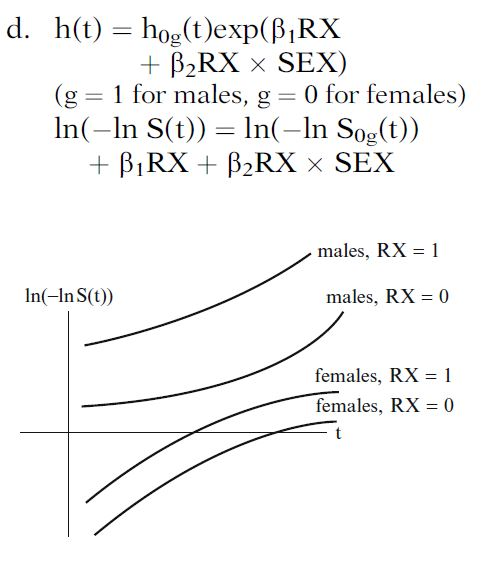
\includegraphics[width =\textwidth, height=5cm]{CH5_G4.JPG}
         d. Interaction and stratification model.
    \end{column}
\end{columns}
\end{block}
\end{frame}

\begin{frame}
\frametitle{The Stratified Cox Likelihood}
\begin{block}{Problem 5.4 - Partial MLE of a SC Model}
Consider the following survival data. Location doesn't satisfy the PH assumption. Assuming no interaction, create an appropriate SC model for this data and estimate the parameters by maximizing the partial likelihood.
\begin{center}
\begin{tabular}{c c c c c} \hline
 Name & Time & Status & Coupon & Location \\ \hline
Barry & 2 & 1 & 1 & 0 \\
 Gary & 3 & 0 & 1 & 0\\
Susan & 5 & 1 & 0 & 0\\
  John & 8 & 1 & 1 & 0\\
  Harry & 3 & 1 & 1 & 1 \\
  Larry & 5 & 1& 1& 1 \\
  David & 7 & 0& 0& 1 \\
\end{tabular}
\end{center}
\end{block}
\end{frame}



\end{document}

